\documentclass{beamer}
\usetheme{ucl}

\usepackage[center]{subfigure}
\usepackage[numbers,sort&compress]{natbib}
\usepackage{hyperref}
\usepackage{tikz}
\usetikzlibrary{arrows.meta, positioning, fit, backgrounds, shapes, arrows, calc, shadows, decorations.pathreplacing}
\usepackage{multirow}
\usepackage{}

%%% Change the color of the main banner
\setbeamercolor{banner}{bg=lightblue,fg=black}

%%% The main structural elements
\setbeamercolor{structure}{fg=black}

%%% Puts the frame title in the banner
\useoutertheme[small]{ucltitlebanner}

%%% Sets the body of block elements to be clear
% \setbeamercolor{block body}{bg=white,fg=black}

%%% Include UCL logo on title slide
% \titlegraphic{\includegraphics[width=0.10\paperwidth]{ucl_logo}}

%%% Include UCL logo in bottom right corner of all slides
% \logo{\includegraphics[width=0.05\paperwidth]{ucl_logo.jpg}}

%%%%%% Some other settings that can make things look nicer
%%% Set a smaller indent for description environment
\setbeamersize{description width=2em}
%%% Remove nav symbols (and shift any logo down to corner)
\setbeamertemplate{navigation symbols}{\vspace{-2ex}}

\title[]{Deep Q-learning for Limit Order Book Trading in Foreign Exchange Markets}
\author[Floris Dobber \and Adam Keys]{Floris Dobber \and Adam Keys}
\institute[UCL]{%
  Department of Computer Science \\ %
  University College London
}
\date{13 September 2024}

\begin{document}

\begin{frame}
  \titlepage
\end{frame}

%% Show footer at the bottom of the slide, but not on the title slide
\setbeamertemplate{footline}[author title date]

\section{Introduction}

\begin{frame}
  \frametitle{Introduction}

  \begin{itemize}
    \item Application of reinforcement learning (RL) to limit order book (LOB) trading in foreign exchange (FX) markets
    \item Reinforcement learning
      \begin{itemize}
        \item Deep Q-Network (DQN) algorithm with double Q-learning, dueling networks, distributional rewards and multi-step returns
        \item Ape-X framework for distributed training
      \end{itemize}
    \item Limit order book simulation
      \begin{itemize}
        \item Agent based model (ABM) simulator (ABIDES)
        \item Simulate entire 10 levels of the LOB based on historical data
      \end{itemize}
    \item Foreign exchange markets
      \begin{itemize}
        \item Largest financial market at \$7.5 trillion daily volume in 2022 \cite{BIS2022triennial}
        \item Focus on EUR/USD as most liquid and traded currency pair 22.7\% of total volume \cite{BIS2022triennial}
      \end{itemize}
  \end{itemize}

\end{frame}

\begin{frame}
  \frametitle{Objectives}

  \begin{itemize}
    \item Develop a realistic simulation of the FX market using the ABIDES-Gym framework, focusing on replicating key stylized facts of the EUR/USD market.
    \item Implement and train deep Q-learning agents to trade in the simulated environment.
    \item Evaluate the agents' performance across various market regimes, comparing it to
  both simple and sophisticated baseline strategies.
    \item Analyze the agents' learned behaviors and trading patterns under different market
  conditions.
  \end{itemize}

\end{frame}

\section{Background}

\begin{frame}
  \frametitle{Background: Deep Q-learning}

  \begin{itemize}
    \item Combines Q-learning with deep neural networks
    \item Enhancements
    \begin{itemize}
      \item Experience replay: Breaks correlations between experiences \cite{mnih2015humanlevel}
      \item Double Q-learning: Improved value estimation accuracy \cite{vanhasselt2015deep}
      \item Dueling networks: Better generalization across actions \cite{wang2016dueling}
      \item Distributional Q-learning: Richer representation of uncertainty \cite{bellemare2017distributional}
      \item Multi-step learning: Faster reward propagation and reduced bias \cite{sutton1998reinforcement}
    \end{itemize}
    \item Ape-X architecture \cite{horgan2018distributed}
    \begin{itemize}
      \item Distributed reinforcement learning framework
      \item Multiple actors generate experiences on CPU cores, central learner updates Q-values via the GPU
      \item Improves learning efficiency and stability
    \end{itemize}
  \end{itemize}
\end{frame}

\begin{frame}
  \frametitle{Background: DQN Network Architecture}


  \begin{figure}[htbp]\centering
    \definecolor{green}{HTML}{55a868}
    \definecolor{blue}{HTML}{4c72b0}
    \resizebox{0.5\textwidth}{!}{
      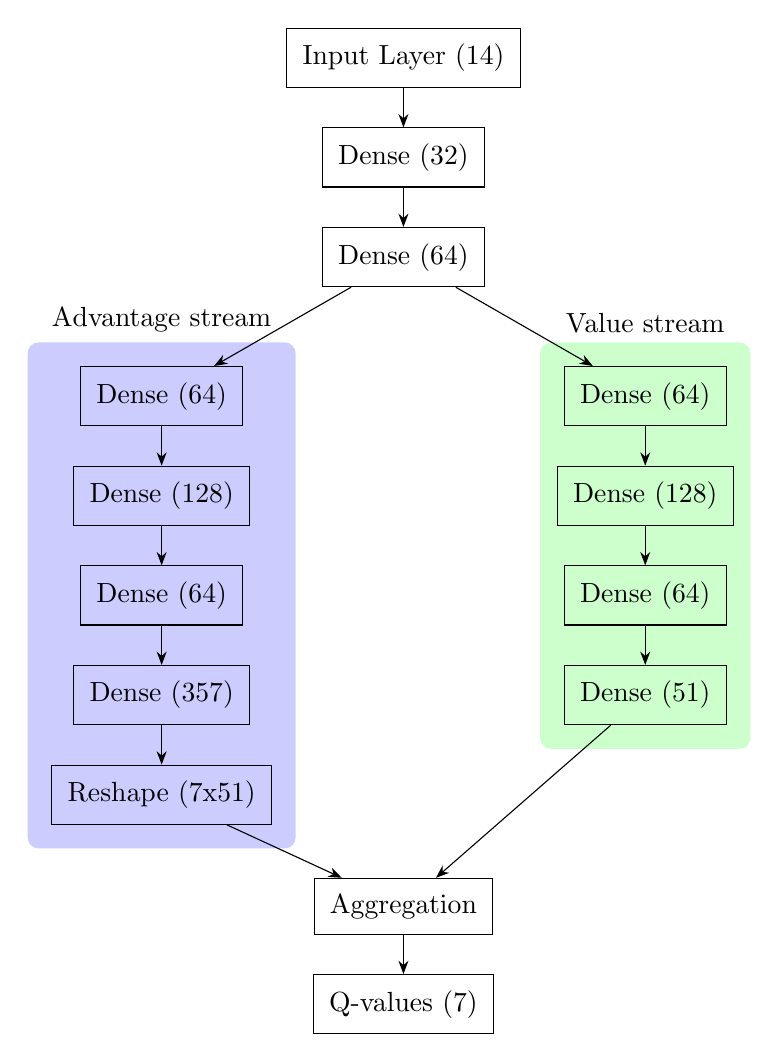
\begin{tikzpicture}[
        layer/.style={rectangle, draw, inner sep=0.2cm},
        >=Stealth
      ]

      % Input Layer
      \node[layer] (input) at (0,0) {Input Layer (14)};  % Equal to state space

      % Base Model - fcnet_hiddens
      \node[layer, below=0.5cm of input] (hidden1) {Dense (32)};
      \node[layer, below=0.5cm of hidden1] (hidden2) {Dense (64)};

      % Advantage stream - hiddens
      \node[layer, below left=1cm and 1cm of hidden2] (a1) {Dense (64)};
      \node[layer, below=0.5cm of a1] (a2) {Dense (128)};
      \node[layer, below=0.5cm of a2] (a3) {Dense (64)};
      \node[layer, below=0.5cm of a3] (a4) {Dense (357)};  % 7x51 = num_actions x num_atoms
      \node[layer, below=0.5cm of a4] (a_reshape) {Reshape (7x51)};  % 7 due to num_actions

      % Value stream - hiddens
      \node[layer, below right=1cm and 1cm of hidden2] (v1) {Dense (64)};
      \node[layer, below=0.5cm of v1] (v2) {Dense (128)};
      \node[layer, below=0.5cm of v2] (v3) {Dense (64)};
      \node[layer, below=0.5cm of v3] (v4) {Dense (51)};  % num_atoms

      % Aggregation
      \node[layer, below=7.5cm of hidden2] (agg) {Aggregation};

      % Final Output
      \node[layer, below=0.5cm of agg] (q1) {Q-values (7)};  % Equal to action space

      % Connections
      \draw[->] (input) -- (hidden1);
      \draw[->] (hidden1) -- (hidden2);
      \draw[->] (hidden2) -- (a1);
      \draw[->] (hidden2) -- (v1);
      \draw[->] (a1) -- (a2);
      \draw[->] (a2) -- (a3);
      \draw[->] (a3) -- (a4);
      \draw[->] (a4) -- (a_reshape);
      \draw[->] (a_reshape) -- (agg);
      \draw[->] (v1) -- (v2);
      \draw[->] (v2) -- (v3);
      \draw[->] (v3) -- (v4);
      \draw[->] (v4) -- (agg);
      \draw[->] (agg) -- (q1);

      % Background rectangles
      \begin{scope}[on background layer]
        \node[fit=(a1) (a_reshape), inner sep=0.3cm, fill=blue!20, label=Advantage stream, rounded corners] {};
        \node[fit=(v1) (v4), inner sep=0.3cm, fill=green!20, label=Value stream, rounded corners] {};
      \end{scope}

      \end{tikzpicture}
    }
  \end{figure}
\end{frame}

\begin{frame}
  \frametitle{Background: Ape-X Architecture}

  \begin{figure}[htbp]
    \centering
    \definecolor{green}{HTML}{55a868}
    \definecolor{blue}{HTML}{4c72b0}
    \definecolor{red}{HTML}{dd8452}
    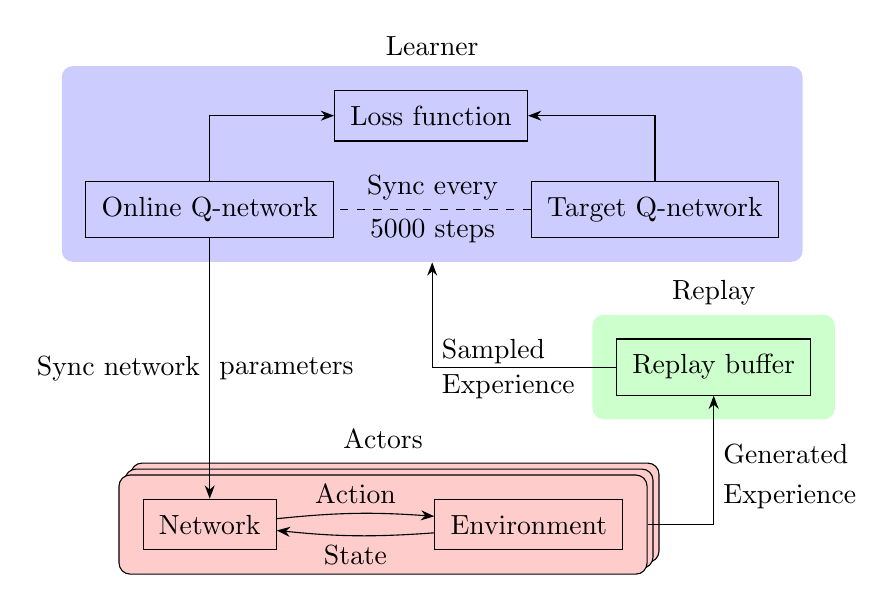
\begin{tikzpicture}[
      scale=0.8,
      layer/.style={rectangle, draw, inner sep=0.2cm},
      box/.style={rectangle, draw, inner sep=0.2cm},
      dcs/.style = {double copy shadow, shadow xshift=3pt, shadow yshift=-3pt},
      >=Stealth
    ]

    % Learner
    \node[box] (online) at (0,0) {Online Q-network};
    \node[box, right=2.5cm of online] (target) {Target Q-network};
    \node[box, above right=0.5cm and 0cm of online] (loss) {Loss function};

    % Replay
    \node[box] (buffer) at (8,-2.5) {Replay buffer};

    % Actors
    \node[box] (actor_network) at (0,-5) {Network};
    \node[box, right=2cm of actor_network] (actor_env) {Environment};

    % Backgrounds
    \begin{scope}[on background layer]
      \node[fit=(target) (online) (loss), inner sep=0.3cm, fill=blue!20, rounded corners, label=Learner] (learner) {};
      \node[fit=(buffer), inner sep=0.3cm, fill=green!20, rounded corners, label=Replay] (replay) {};
      \node[box, dcs, fit=(actor_network) (actor_env), inner sep=0.3cm, fill=red!20, rounded corners, label={[yshift=0.2cm]Actors}] (actors) {};
    \end{scope}

    % Connections
    \draw[dashed] (target) -- node[above] {Sync every} node[below] {5000 steps} (online);
    \draw[->] (buffer) -| node[right, yshift=0.2cm] {Sampled} node[right, yshift=-0.25cm] {Experience} (learner);
    \draw[->] (online) -- node[left] {Sync network} node[right] {parameters} (actor_network);
    \draw[->] (actors) -| node[right, yshift=0.9cm] {Generated} node[right, yshift=0.35cm] {Experience} (buffer);
    \draw[->] (actor_network) to[bend left=5] node[above] {Action} (actor_env);
    \draw[->] (actor_env) to[bend left=5] node[below] {State} (actor_network);
    \draw[->] (online) |- (loss);
    \draw[->] (target) |- (loss);

    \end{tikzpicture}
  \end{figure}
\end{frame}

\begin{frame}
  \frametitle{Background: Limit Order Book Simulation}

  \begin{itemize}
    \item Agent-Based Models (ABMs)
    \begin{itemize}
      \item Bottom-up approach to market simulation
      \item Captures complex market dynamics from agent interactions
    \end{itemize}
    \item ABIDES Framework \cite{byrd2020abides}
    \begin{itemize}
      \item Agent-Based Interactive Discrete Event Simulation
      \item Simulates high-fidelity market environments
      \item Includes Gym interface for RL integration
    \end{itemize}
    \item Key Features
    \begin{itemize}
      \item Reproduces heavy-tailed return distributions
      \item Captures volatility clustering
      \item Models market impact effectively
    \end{itemize}
    \item Advantages for Research
    \begin{itemize}
      \item Controllable and reproducible experiments
      \item Ability to test strategies without real capital risk
      \item Facilitates study of market microstructure
    \end{itemize}
  \end{itemize}

\end{frame}

\section{Methodology}

\begin{frame}
  \frametitle{Methodology: Environment}

  \begin{itemize}
    \item Episode Structure
    \begin{itemize}
      \item 1-hour duration, 0.2-second time steps (18,000 steps/episode)
    \end{itemize}
    \item State Space
    \begin{itemize}
      \item 14 dimensions including time, cash, inventory, market data
      \item Directional signal as probability distribution over price movements
    \end{itemize}
    \item Action Space
    \begin{itemize}
      \item 7 discrete actions: buy/sell at 3 price levels + skip
      \item Maximum inventory constraint of 10 units
    \end{itemize}
    \item Reward Function
    \begin{itemize}
      \item Combination of directional reward and profit-and-loss
      \item Curriculum learning approach with shifting weights
    \end{itemize}
    \item Background Agents
    \begin{itemize}
      \item Market makers, value agents, momentum agents, noise agents
      \item Creates realistic market dynamics and liquidity
    \end{itemize}
  \end{itemize}
\end{frame}

\begin{frame}{Methodology: Synthetic Alpha Signal}
    \begin{gather*}
    \hat{p}_t = w\hat{p}_{t-1} + (1 - w)d_t, \hspace{1em}w\in (0,1) \\
    d_t \sim \text{Dir}(\alpha(\bar{r}_{t+h})) \\
    \bar{r}_{t+h} = \frac{\bar{x}_{t+h}-x_t}{x_t}, \hspace{0.8em} \text{where} \hspace{0.8em} \bar{x}_{t+h} = \frac{1}{h}\sum_{i=1}^h x_{t+i}
    \end{gather*}
    Signal parameterized such that probability mass is concentrated on dimension indicating future price move:
    $$
    \alpha(\bar{r}_{t+h}) = 
    \begin{cases}
    (a^H, a^L, a^L), \hspace{0.5em} \text{if}\hspace{0.5em} \bar{r}_{t+h} < -k\\
    (a^L, a^H, a^L), \hspace{0.5em} \text{if}\hspace{0.5em} |\bar{r}_{t+h}| \le k\\
    (a^L, a^L, a^H), \hspace{0.5em} \text{if}\hspace{0.5em} \bar{r}_{t+h} > k\\
    \end{cases}$$
    $$
    a^H, a^L \in \mathbb{R^+} \hspace{0.7em} \text{where} \hspace{0.7em} a^H > a^L
    $$
        
    \end{frame}
    
    \begin{frame}{Methodology: Reward Function}
    
    \begin{align*}
        \text{Portfolio Value}& \hspace{1.7em} {PV}_t = C_t + I_tx_t\\
        \text{P\&L Reward}&\hspace{1.7em} r^{P\&L}_{t+1} = {PV}_t - {PV}_{t-1}\\
        \text{Directional Reward}& \hspace{1.7em} r^{dir}_{t+1} = \kappa [-1,0,1]\cdot \hat{p}_t I_t\\
        \text{Total Reward}& \hspace{1.7em} R_{t+1} = \phi r^{\text{dir}}_{t+1} + (1 - \phi)r^{\text{P\&L}}_{t+1}\\
    \end{align*}
    $C_t$ denotes cash, $I_t$ inventory holdings, $x_t$ is the midprice, $\kappa \in \mathbb{R^+}$, and $\hat{p}_t$ is the alpha signal.\\
    \vspace{1em}
    After each step, the directional weight ($\phi_0 = 1$) reduces by some scalar factor:
    $$\phi \leftarrow \gamma\phi, \hspace{2em}\gamma\in(0,1)$$
    \end{frame}

\begin{frame}
  \frametitle{Methodology: Agent}

  \begin{itemize}
    \item Ape-X Distributed Architecture
    \begin{itemize}
      \item 4 actors, each running 4 parallel environments
    \end{itemize}
    \item Training Parameters
    \begin{itemize}
      \item Total training steps: 3,000,000
      \item Buffer size: 200,000 experiences
      \item Learning rate: 5e-6 (static)
      \item Discount factor (gamma): 0.99
      \item Target network update frequency: 5000 steps
      \item Multi-step learning with n=10
    \end{itemize}
  \end{itemize}
\end{frame}

\begin{frame}
  \frametitle{Methodology: Baseline Agents}

  \begin{itemize}
    \item Random Agent
    \begin{itemize}
      \item Selects actions uniformly at random
      \item Establishes lower performance bound
    \end{itemize}
    \item Buy-and-Hold Agent
    \begin{itemize}
      \item Buys fixed amount at start, holds until end
      \item Provides simple profit baseline
    \end{itemize}
    \item Aggressive Agent
    \begin{itemize}
      \item Crosses spread to place limit orders
      \item Uses directional signal to inform trading decisions
    \end{itemize}
    \item Common Constraints
    \begin{itemize}
      \item Maximum inventory size of 10 units
    \end{itemize}
  \end{itemize}

\end{frame}

\begin{frame}
  \frametitle{Motivations}

  \begin{block}
    {Research Questions}
    \begin{itemize}
      \item Can a deep Q-learning agent learn effective trading strategies in a simulated FX market environment?
      \item To what extent can the RL agents adapt their strategy to various market conditions, such as high volatility, trends, and price jumps?
    \end{itemize}
  \end{block}

\end{frame}

\begin{frame}
  \frametitle{Experimental Setup}

  \begin{itemize}
    \item 8 distinct market regimes identified
    \begin{itemize}
      \item High volatility, Low volatility
      \item Upward trend, Downward trend, No trend
      \item Upward jump, Downward jump
      \item Mixed (combination of all regimes)
    \end{itemize}
    \item Training Process
    \begin{itemize}
      \item One agent trained per regime
      \item 35 one-hour episodes per regime for training
    \end{itemize}
    \item Evaluation
    \begin{itemize}
      \item 7 one-hour episodes per regime for testing
      \item Each agent tested across all 8 regimes
    \end{itemize}
    \item Performance Metrics
    \begin{itemize}
      \item Returns and excess returns
      \item Sharpe ratio
      \item Maximum drawdown
      \item Action frequency and trading style analysis
    \end{itemize}
  \end{itemize}

\end{frame}

\section{Results}

\begin{frame}
  \frametitle{Results: Selected Training Periods}

  \begin{figure}
    \centering
    \subfigure[High Volatility]{\includegraphics[width=0.3\textwidth]{figures/high_vol_training_period.png}}
    \subfigure[Upward Trend]{\includegraphics[width=0.3\textwidth]{figures/trend_up_training_period.png}}
    \subfigure[Upward Jump]{\includegraphics[width=0.3\textwidth]{figures/jump_up_training_period.png}}
    \subfigure[Low Volatility \linebreak No Trend]{\includegraphics[width=0.3\textwidth]{figures/no_trend_training_period.png}}
    \subfigure[Downward Trend]{\includegraphics[width=0.3\textwidth]{figures/trend_down_training_period.png}}
    \subfigure[Downward Jump]{\includegraphics[width=0.3\textwidth]{figures/jump_down_training_period.png}}
  \end{figure}
\end{frame}

\begin{frame}
  \frametitle{Results: Environment Analysis}

  \begin{figure}
    \centering
    \includegraphics[width=0.7\textwidth]{figures/hist_vs_sim_prices.png}
    \caption{Comparison of historical and simulated prices.}
  \end{figure}

  \begin{itemize}
    \item Simulated prices closely match historical data
  \end{itemize}

\end{frame}

\begin{frame}
  \frametitle{Results: Environment Analysis II}

  \begin{figure}
    \centering
    \subfigure[Log Return Distribution]{\includegraphics[width=0.39\textwidth]{figures/log_returns_hist.png}}
    \subfigure[Return Autocorrelation]{\includegraphics[width=0.39\textwidth]{figures/returns_autocorr.png}}
    \subfigure[Volatility Autocorrelation]{\includegraphics[width=0.39\textwidth]{figures/volatility_autocorr.png}}
    \subfigure[Inter-arrival Times]{\includegraphics[width=0.39\textwidth]{figures/time_between_ticks_100sec.png}}
  \end{figure}
\end{frame}

\begin{frame}
  \frametitle{Results: Training Performance \small{(High Volatility)}}

  \begin{figure}
    \setcounter{subfigure}{0}
    \centering

    \subfigure[Reward Weight]{\includegraphics[width=0.4\textwidth]{figures/high_vol_training_weights.png}}
    \subfigure[Reward]{\includegraphics[width=0.4\textwidth]{figures/high_vol_training_reward.png}}
    \subfigure[Entropy]{\includegraphics[width=0.4\textwidth]{figures/high_vol_training_entropy.png}}
    \subfigure[TD Error / Loss]{\includegraphics[width=0.4\textwidth]{figures/high_vol_training_td_error.png}}
  \end{figure}

  \begin{itemize}
    \item Transition from directional to profit-based reward
  \end{itemize}
\end{frame}

\begin{frame}
  \frametitle{Results: Baseline Strategies Returns}

  \begin{table}[htbp]
    \fontsize{7}{9}\selectfont
    \centering
    \caption{Average return per episode for the baseline strategies across market regimes. The values represent the average percentage return per episode (one hour) in the testing set.}
    \begin{tabular}{l|rrrrrrrr|r}
    \hline
    \multirow{2}{*}{Agent} & \multicolumn{8}{c|}{Market Type} & \multirow{2}{*}{Agent Avg.} \\
    \cline{2-9}
    & HV &  LV &  UT &  DT &  NT &  UJ &  DJ & MX \\
    \hline
    Random       &     -0.08 &    -0.05 &     -0.13 &       -0.05 &     -0.05 &    -0.14 &      -0.02 &  -0.10 &       -0.08 \\
    Buy and Hold &      0.05 &    -0.01 &      0.09 &       -0.11 &     -0.01 &     0.07 &      -0.08 &   0.01 &        0.00 \\
    Aggressive   &      \textbf{0.86} &     \textbf{0.38} &      \textbf{0.35} &        \textbf{0.46} &      \textbf{0.36} &     \textbf{0.45} &       \textbf{0.51} &   \textbf{0.65} &        \textbf{0.50} \\
    \hline
    Market Avg.  &      0.28 &     0.11 &      0.10 &        0.10 &      0.10 &     0.12 &       0.14 &   0.19 &        0.14 \\
    \end{tabular}
  \end{table}
  
  \begin{itemize}
    \item Environments are challenging for simple strategies
    \item Aggressive agent outperforms other baselines in all market regimes
  \end{itemize}
  
\end{frame}

\begin{frame}
  \frametitle{Results: Returns}

  \begin{table}[htbp]
    \fontsize{7}{9}\selectfont
    \centering
    \caption{Average return per episode for each agent in different market conditions. The values represent the average percentage return per episode (one hour) in the testing set.}
    \begin{tabular}{l|rrrrrrrr|r}
    \hline
    \multirow{2}{*}{Agent} & \multicolumn{8}{c|}{Market Type} & \multirow{2}{*}{Agent Avg.} \\
    \cline{2-9}
    & HV &  LV &  UT &  DT &  NT &  UJ &  DJ & MX \\
    \hline
    High volatility &      0.42 &     0.16 &      0.19 &        0.19 &      0.17 &     0.23 &       \textbf{0.24} &   \textbf{0.31} &        0.24 \\
    Low volatility  &      0.17 &     0.11 &      0.11 &        0.12 &      0.10 &     0.10 &       0.11 &   0.11 &        0.12 \\
    Upward trend    &      0.21 &     0.12 &      0.13 &        0.14 &      0.13 &     0.14 &       0.12 &   0.14 &        0.14 \\
    Downward trend  &      0.33 &     0.17 &      0.19 &        0.18 &      0.18 &     0.20 &       0.19 &   0.28 &        0.21 \\
    No trend        &      0.39 &     \textbf{0.26} &      \textbf{0.21} &        \textbf{0.23} &      \textbf{0.22} &     0.21 &       \textbf{0.24} &   0.30 &        \textbf{0.26} \\
    Upward jump     &      0.41 &     0.19 &      0.18 &        \textbf{0.23} &      0.19 &     \textbf{0.25} &       0.18 &   0.25 &        0.24 \\
    Downward jump   &      \textbf{0.48} &     0.10 &      0.11 &        0.11 &      0.10 &     0.13 &       0.12 &   0.20 &        0.17 \\
    Mixed           &      0.21 &     0.11 &      0.10 &        0.12 &      0.08 &     0.12 &       0.16 &   0.16 &        0.13 \\
    \hline
    Market Avg.     &      0.33 &     0.15 &      0.15 &        0.16 &      0.15 &     0.17 &       0.17 &   0.22 &        0.19 \\
    \end{tabular}
  \end{table}

  \begin{itemize}
    \item All agents consistently achieve positive returns
    \item High volatility is the most profitable regime, rest are similar
    \item No agent beat the aggressive baseline return
  \end{itemize}
  
\end{frame}

\begin{frame}
  \frametitle{Results: Sharpe Ratio}

  \begin{table}[htbp]
    \fontsize{7}{9}\selectfont
    \centering
    \caption{Annualized Sharpe ratio for each agent in different market regimes. The values represent the annualized Sharpe ratio assuming a risk-free rate of zero.}
    \begin{tabular}{l|rrrrrrrr|r}
    \hline
    \multirow{2}{*}{Agent} & \multicolumn{8}{c|}{Market Type} & \multirow{2}{*}{Agent Avg.} \\
    \cline{2-9}
    & HV &  LV &  UT &  DT &  NT &  UJ &  DJ & MX \\
    \hline
    High volatility &      \textbf{3.48} &     2.21 &      2.79 &        2.55 &      2.34 &     2.64 &       3.05 &   \textbf{3.34} &        2.80 \\
    Low volatility  &      0.99 &     \textbf{3.65} &      2.96 &        3.31 &      \textbf{3.20} &     \textbf{3.23} &       3.03 &   2.65 &        2.88 \\
    Upward trend    &      1.76 &     2.17 &      2.76 &        2.78 &      2.67 &     2.88 &       2.26 &   2.57 &        2.48 \\
    Downward trend  &      1.39 &     2.57 &      2.16 &        2.33 &      2.64 &     2.41 &       2.36 &   2.42 &        2.29 \\
    No trend        &      1.95 &     2.64 &      2.46 &        2.20 &      2.43 &     2.14 &       2.47 &   2.45 &        2.34 \\
    Upward jump     &      3.08 &     2.60 &      2.95 &        2.70 &      2.94 &     2.79 &       2.37 &   3.10 &        2.82 \\
    Downward jump   &      1.82 &     3.24 &      \textbf{3.66} &        \textbf{3.84} &      2.70 &     2.74 &       \textbf{3.49} &   2.67 &        \textbf{3.02} \\
    Mixed           &      2.72 &     2.69 &      2.78 &        2.94 &      2.30 &     2.76 &       2.95 &   2.74 &        2.73 \\
    \hline
    Market Avg.     &      2.15 &     2.72 &      2.82 &        2.83 &      2.65 &     2.70 &       2.75 &   2.74 &        2.67 \\
    \end{tabular}
  \end{table}

  \begin{itemize}
    \item All agents surpassed the aggressive baseline Sharpe ratio of 1.43
    \item Demonstrates robust risk management capabilities in all agents
  \end{itemize}
  
\end{frame}

\begin{frame}
  \frametitle{Results: Excess Returns}

  \begin{table}[htbp]
    \fontsize{7}{9}\selectfont
    \centering
    \caption{Average excess return per episode for each agent in different market regimes. The values represent the average percentage excess return per episode (one hour) in the testing set.}
    \begin{tabular}{l|rrrrrrrr|r}
    \hline
    \multirow{2}{*}{Agent} & \multicolumn{8}{c|}{Market Type} & \multirow{2}{*}{Agent Avg.} \\
    \cline{2-9}
    & HV &  LV &  UT &  DT &  NT &  UJ &  DJ & MX \\
    \hline
    High volatility &      0.32 &     0.17 &      0.02 &        0.38 &      0.18 &     0.11 &       \textbf{0.38} &   \textbf{0.27} &        0.23 \\
    Low volatility  &      0.07 &     0.13 &     -0.06 &        0.31 &      0.11 &    -0.03 &       0.20 &   0.04 &        0.10 \\
    Upward trend    &      0.11 &     0.14 &     -0.05 &        0.31 &      0.13 &     0.02 &       0.25 &   0.11 &        0.13 \\
    Downward trend  &      0.23 &     0.19 &      0.02 &        0.37 &      0.19 &     0.09 &       0.32 &   0.24 &        0.21 \\
    No trend        &      0.29 &     \textbf{0.27} &      \textbf{0.04} &        0.42 &      \textbf{0.22} &     0.08 &       0.37 &   0.26 &        \textbf{0.24} \\
    Upward jump     &      0.32 &     0.20 &      0.02 &        \textbf{0.43} &      0.20 &     \textbf{0.13} &       0.32 &   0.22 &        0.23 \\
    Downward jump   &      \textbf{0.38} &     0.12 &     -0.05 &        0.30 &      0.11 &     0.00 &       0.26 &   0.18 &        0.16 \\
    Mixed           &      0.10 &     0.13 &     -0.07 &        0.31 &      0.09 &     0.00 &       0.30 &   0.13 &        0.12 \\
    \hline
    Market Avg.     &      0.23 &     0.17 &     -0.02 &        0.35 &      0.16 &     0.05 &       0.30 &   0.18 &        0.18 \\
    \end{tabular}
  \end{table}

  \begin{itemize}
    \item Correlation between returns and market returns is 0.178
    \item The aggressive baseline had 0.17\% excess return in UT
  \end{itemize}
  
\end{frame}

\begin{frame}
  \frametitle{Results: Trading Style}

  \begin{figure}
    \centering
    \includegraphics[width=0.75\textwidth]{figures/action_heatmap.png}
  \end{figure}

  \begin{itemize}
    \item Agents exhibit a passive trading style, skip most frequently
    \item Some variation in trading style across agents
  \end{itemize}

\end{frame}

\begin{frame}
  \frametitle{Results: Trading Style II}

  \begin{figure}
    \centering
    \includegraphics[width=0.75\textwidth]{figures/regime_action_heatmap.png}
  \end{figure}

  \begin{itemize}
    \item Minor differences in trading style across market regimes
    \item Same pattern can be seen for individual agents
  \end{itemize}

\end{frame}

\begin{frame}
  \frametitle{Results: Position Analysis}

  \begin{figure}
    \centering
    \setcounter{subfigure}{0}
    \subfigure[Average Position Size]{\includegraphics[width=0.45\textwidth]{figures/avg_position_size.png}}
    \subfigure[Average Position Duration]{\includegraphics[width=0.45\textwidth]{figures/avg_position_duration.png}}
  \end{figure}

  \begin{itemize}
    \item Agents maintain small position sizes and short holding periods
    \item Conservative trading style with limited exposure
    \item Aggressive agent: 9.11 average size and 60 sec average duration
    \item Pearson correlation between position size and returns is 0.52
  \end{itemize}

\end{frame}

\section{Conclusion}

\begin{frame}
  \frametitle{Conclusions and Future Work}

  \begin{block}{Conclusions}
    \begin{itemize}
      \item Deep Q-learning agents can learn profitable, uncorrelated trading strategies in simulated FX markets
      \item Agents demonstrate superior risk-adjusted returns compared to baselines
      \item Conservative trading style with short holding periods and small positions
      \item Limited adaptability to changing market conditions during execution
    \end{itemize}
  \end{block}

  \begin{block}{Future Work}
    \begin{itemize}
      \item Implement more sophisticated curriculum learning approaches
      \item Develop automated methods to improve simulation fidelity
      \item Expand action space to allow deeper order book interactions
    \end{itemize}
  \end{block}
\end{frame}

\section{Acknowledgements}

\begin{frame}
  \frametitle{Acknowledgements}

  \begin{itemize}
    \item Dr Paris Pennesi
    \item Dr Pawel Chilinski
    \item Dr Riccardo Della Vecchia
  \end{itemize}
\end{frame}

\begin{frame}[allowframebreaks]
  \frametitle{References}
  \bibliographystyle{IEEEtranN}
  \bibliography{references}
\end{frame}

\appendix

\begin{frame}
  \frametitle{Appendix: Training Performance \small{(Upward Trend)}}

  \begin{figure}
    \setcounter{subfigure}{0}
    \centering

    \subfigure[Reward Weight]{\includegraphics[width=0.4\textwidth]{figures/trend_up_training_weights.png}}
    \subfigure[Reward]{\includegraphics[width=0.4\textwidth]{figures/trend_up_training_reward.png}}
    \subfigure[Entropy]{\includegraphics[width=0.4\textwidth]{figures/trend_up_training_entropy.png}}
    \subfigure[TD Error / Loss]{\includegraphics[width=0.4\textwidth]{figures/trend_up_training_td_error.png}}
  \end{figure}
\end{frame}

\begin{frame}
  \frametitle{Appendix: Baseline Strategies Excess Returns}

  \begin{table}[htbp]
    \fontsize{7}{9}\selectfont
    \centering
    \caption[Baseline Strategies Excess Return]{Average excess return for the baseline strategies across market regimes. The values represent the average percentage excess return in the testing set.}
    \begin{tabular}{l|rrrrrrrr|r}
    \hline
    \multirow{2}{*}{Agent} & \multicolumn{8}{c|}{Market Type} & \multirow{2}{*}{Agent Avg.} \\
    \cline{2-9}
    & HV &  LV &  UT &  DT &  NT &  UJ &  DJ & MX \\
    \hline
    Random       &     -0.18 &    -0.03 &     -0.30 &        0.14 &     -0.03 &    -0.26 &       0.12 &  -0.14 &       -0.09 \\
    Buy and Hold &     -0.05 &     0.00 &     -0.08 &        0.08 &      0.00 &    -0.06 &       0.06 &  -0.02 &       -0.01 \\
    Aggressive   &      0.76 &     0.38 &      0.17 &        0.66 &      0.37 &     0.32 &       0.66 &   0.60 &        0.49 \\
    \hline
    Market Avg.  &      0.18 &     0.12 &     -0.07 &        0.29 &      0.11 &     0.00 &       0.28 &   0.15 &        0.13 \\
    \end{tabular}
  \end{table}
\end{frame}

\begin{frame}
  \frametitle{Appendix: Baseline Strategies Sharpe Ratios}

  \begin{table}[htbp]
    \fontsize{7}{9}\selectfont
    \centering
    \caption[Baseline Strategies Sharpe Ratio]{Average Sharpe ratio for the baseline strategies across market regimes. The values represent the average Sharpe ratio in the testing set.}
    \begin{tabular}{l|rrrrrrrr|r}
    \hline
    \multirow{2}{*}{Agent} & \multicolumn{8}{c|}{Market Type} & \multirow{2}{*}{Agent Avg.} \\
    \cline{2-9}
    & HV &  LV &  UT &  DT &  NT &  UJ &  DJ & MX \\
    \hline
    Random       &     -0.13 &    -0.24 &     -0.62 &       -0.26 &     -0.25 &    -0.68 &      -0.10 &  -0.34 &       -0.33 \\
    Buy and Hold &      0.06 &    -0.03 &      0.27 &       -0.34 &     -0.02 &     0.18 &      -0.19 &   0.04 &       0.00 \\
    Aggressive   &      1.94 &     1.02 &      1.05 &        1.39 &      1.24 &     1.30 &       1.61 &   1.89 &        1.43 \\
    \hline
    Market Avg.  &      0.63 &     0.25 &      0.24 &        0.26 &      0.32 &     0.27 &       0.44 &   0.53 &        0.37 \\
    \end{tabular}
    \label{tab:baseline_sharpe_ratio}
  \end{table}
\end{frame}

\begin{frame}
  \frametitle{Appendix: Baseline Strategies Max Drawdown}

  \begin{table}[htbp]
    \fontsize{7}{9}\selectfont
    \centering
    \caption[Baseline Strategies Max Drawdown]{Average maximum drawdown for the baseline strategies across market regimes. The values represent the average maximum drawdown in the testing set.}
    \begin{tabular}{l|rrrrrrrr|r}
    \hline
    \multirow{2}{*}{Agent} & \multicolumn{8}{c|}{Market Type} & \multirow{2}{*}{Agent Avg.} \\
    \cline{2-9}
    & HV &  LV &  UT &  DT &  NT &  UJ &  DJ & MX \\
    \hline
    Random       &     -0.22 &    -0.09 &     -0.16 &       -0.11 &     -0.10 &    -0.17 &      -0.11 &  -0.17 &       -0.14 \\
    Buy and Hold &     -0.19 &    -0.06 &     -0.06 &       -0.13 &     -0.08 &    -0.10 &      -0.15 &  -0.14 &       -0.11 \\
    Aggressive   &     -0.14 &    -0.07 &     -0.06 &       -0.06 &     -0.05 &    -0.07 &      -0.06 &  -0.07 &       -0.07 \\
    \hline
    Market Avg.  &     -0.18 &    -0.07 &     -0.09 &       -0.10 &     -0.07 &    -0.11 &      -0.10 &  -0.13 &       -0.11 \\
    \end{tabular}
    \label{tab:baseline_max_drawdown}
  \end{table}

\end{frame}

\begin{frame}
  \frametitle{Appendix: Max Drawdown}

  \begin{table}[htbp]
    \fontsize{7}{9}\selectfont
    \centering
    \caption[Maximum Drawdown]{Maximum drawdown for each agent in different market regimes. The maximum drawdown is the largest loss an agent would have experienced during a single episode (one hour). The values represent the maximum drawdown in percentage points.}
    \begin{tabular}{l|rrrrrrrr|r}
    \hline
    \multirow{2}{*}{Agent} & \multicolumn{8}{c|}{Market Type} & \multirow{2}{*}{Agent Avg.} \\
    \cline{2-9}
    & HV &  LV &  UT &  DT &  NT &  UJ &  DJ & MX \\
    \hline
    High volatility &     -0.04 &    -0.01 &     -0.02 &       -0.01 &     -0.01 &    -0.01 &      -0.02 &  -0.02 &       -0.02 \\
    Low volatility  &     -0.07 &    -0.01 &     -0.01 &       -0.01 &     -0.01 &    -0.01 &      -0.02 &  -0.02 &       -0.02 \\
    Upward trend    &     -0.05 &    -0.01 &     -0.01 &       -0.01 &     -0.01 &    -0.01 &      -0.02 &  -0.02 &       -0.02 \\
    Downward trend  &     \textbf{-0.13} &    -0.01 &     \textbf{-0.03} &       -0.02 &     -0.01 &    \textbf{-0.03} &      -0.03 &  -0.03 &       \textbf{-0.04} \\
    No trend        &     -0.07 &    \textbf{-0.02} &     -0.01 &       -0.02 &     -0.01 &    -0.03 &      -0.03 &  \textbf{-0.04} &       -0.03 \\
    Upward jump     &     -0.04 &    -0.01 &     -0.01 &       -0.02 &     -0.01 &    -0.01 &      \textbf{-0.04} &  -0.02 &       -0.02 \\
    Downward jump   &     -0.08 &    -0.01 &     -0.01 &       -0.01 &     -0.01 &    -0.02 &      -0.01 &  -0.03 &       -0.02 \\
    Mixed           &     -0.02 &    -0.01 &     -0.01 &       -0.01 &     -0.01 &    -0.01 &      -0.01 &  -0.01 &       -0.01 \\
    \hline
    Market Avg.     &     -0.06 &    -0.01 &     -0.01 &       -0.01 &     -0.01 &    -0.02 &      -0.02 &  -0.02 &       -0.02 \\
    \end{tabular}
  \end{table}
\end{frame}

\end{document}
